\chapter{時系列ユーザビリティ評価システムの提案}
\label{chap:sequential}

\section{評価システムの設計・開発}

\subsection{時系列ストレスグラフ}

\subsection{観察ビデオとのマッピング}

\section{評価システムの有効性についての実験}

\subsection{対象と手続き}

\begin{figure}[htbp]
  \begin{minipage}{0.5\hsize}
    \begin{center}
       \fbox{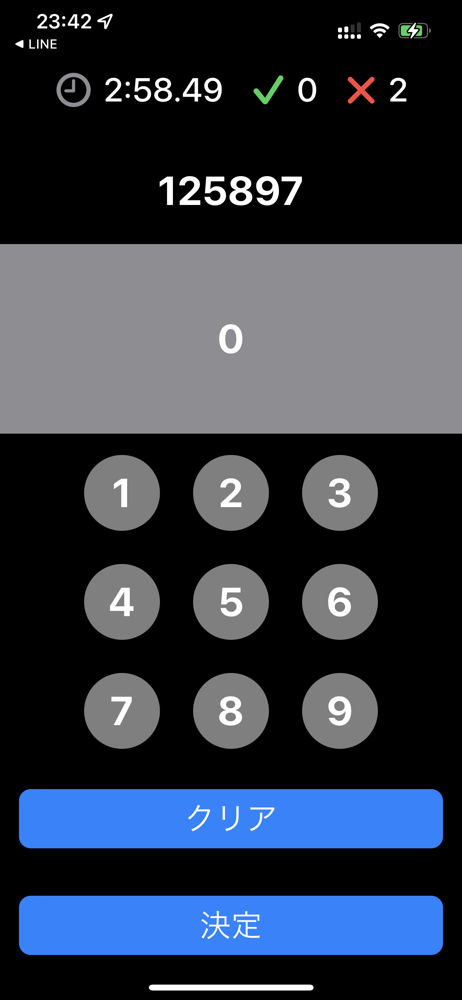
\includegraphics[width=40mm]{new1.png}}
    \end{center}
    \caption{実験マテリアル:テンキー}
    \label{fig:lyspect}
  \end{minipage}
  \begin{minipage}{0.5\hsize}
    \begin{center}
       \fbox{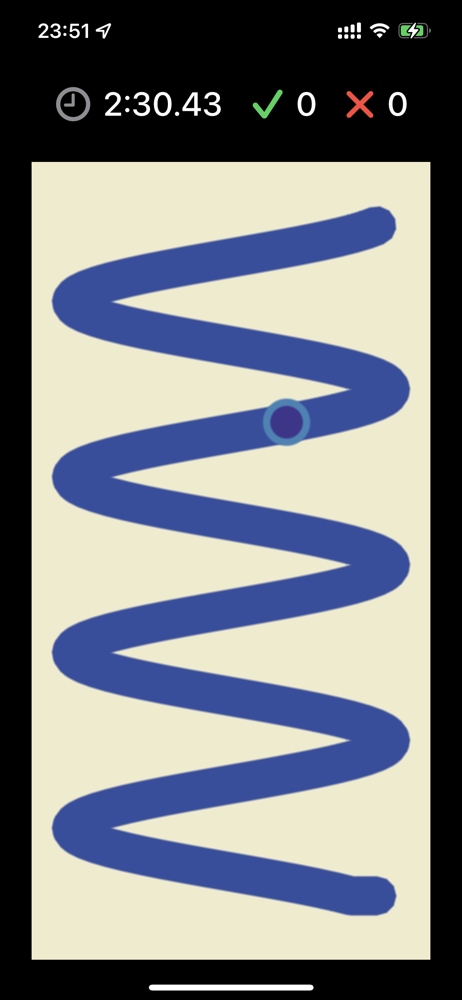
\includegraphics[width=40mm]{new2.png}}
    \end{center}
    \caption{実験マテリアル:ドラッグ}
    \label{fig:lyspect}
  \end{minipage}
\end{figure}


\subsection{結果と考察}